
\chapter{Multivariate Analysis in Metabolomics}

\begin{quote}
{\it Essentially, all models are wrong, but some are useful.}
\\\\
 -- George E. P. Box
\end{quote}

\section{Introduction}

\begin{doublespace}
The applications of chemometrics are as broad as the field of chemistry itself,
but one particularly challenging subdiscipline of bioanalytical chemistry --
known as ``metabolomics'' -- has recently renewed interest in the use of
chemometrics \cite{worley:cmb2013}. Indeed, the chemical complexity of
systems studied by metabolomics {\it necessitates} the use of chemometric
techniques: if metabolomics were a nail, chemometrics would surely be a hammer.
\\\\
Metabolomics is defined \cite{lindon:cmr2000} as ``the quantitative
measurement of the multiparametric metabolic response of living systems to
pathophysiological stimuli or genetic modification.'' Such a definition implies
that metabolomics studies offer the finest-grained detail available in the
nascent field of systems biology: a molecular-level convolution of all upstream
genomic, transcriptomic and proteomic responses of an organism to a given
stimulus or change
\cite{kell:opin2004,trethewey:opin2001,weckwerth:arpb2003}. Metabolites
are the end product of all cellular processes, and their in vivo
concentrations are a direct result of enzymatic activity. While a change in the
expression level of a protein or its coding gene may not necessarily correlate
directly with the activity of that protein, alterations in metabolite
concentrations {\it are} the consequence of altered activity
\cite{terkuile:febs2001}. Thus, metabolites are more proximal to a
phenotype or disease state than either genetic or proteomic information. The
richness of phenotypic information offered by metabolomics has been leveraged
to identify disease biomarkers
\cite{gebregiworgis:cchts2012,vinayavekhin:acscb2010}, to aid in
the drug discovery process \cite{powers:mrc2009,wilcoxen:eodd2010}, and to
study plants \cite{hall:pcell2002}, bacteria
\cite{zhang:jiomic2013,tang:cgen2011}, nutrition
\cite{mcniven:jnb2011}, and the environment
\cite{bundy:metab2009}, among numerous other applications
\cite{baker:nmeth2011}.
\\\\
The rich information promised by metabolomics does not come without a price,
and metabolomics experiments are plagued with difficulty. The number of
small-molecule metabolites in a biofluid, cell lysate, tissue or organ differs
wildly depending on the organism studied, ranging from several hundred to
hundreds of thousands \cite{dunn:trac2005}. While databases of commonly
encountered metabolites have been compiled
\cite{wishart:nar2007,cui:nbiot2008,kind:anchem2009}, they are by no
means complete. Therefore, it is common to encounter unknown signals during
data analysis, complicating the interpretation of metabolic changes between
experimental groups. Metabolite identification is further complicated by a
lack of NMR or mass spectral reference information for known metabolites.
Finally, the diversity of chemical and physical properties of metabolites
makes true simultaneous quantitation of all metabolites present in a system
unattainable with current instrumental capabilities
\cite{lindon:cmr2000,dunn:trac2005,dettmer:msr2007}. As an illustration,
due to the limited molecular mass distribution of the metabolome, comprehensive
metabolomic analyses by mass spectrometry generally require the prefixing of
one or more chromatographic separations prior to analyte ionization
\cite{kell:opin2004,viswanadhan:acsccc2011}.
\\\\
The extraction of information from data in metabolomics experiments is further
complicated by the inherent variability present within each sample. Every
single cell, tissue, organ or organism is fundamentally unique
\cite{rubakhin:nmeth2011}, despite any features (disease state, drug
treatment, {\it etc.}) it may have in common with others of its kind. Thus,
the differentiation between two experimental groups in a metabolomics
experiment requires the identification of relatively few defining or
discriminating chemical features against a large, complex background of
metabolites \cite{wishart:nar2007}. Ideally, these few chemical features
may be identified as a unique set of metabolites that are directly related to
the defining biochemical states of each experimental group. Unfortunately, all
biological systems are easily perturbed by experimental or environmental
factors, including age, gender, diet, cell growth phase, nutrient availability,
pH and temperature \cite{tyagi:ijpsrr2010,zhang:jiomic2013}. Variations in
sample handling procedures, including cell lysis, metabolic quenching,
metabolite extraction and sample storage can also introduce further variability
into the measured data. Finally, variations in signal position, intensity and
shape may manifest from instrumental instabilities on a per-sample basis.
Each of these numerous sources of sample variability increases the magnitude of
$\mathbf{E}$ in any chemometric model that may be applied to the data
(cf. \hyperlink{section.1.1}{Section 1.1}), which decreases the statistical
validity of $f(\mathbf{D})$. Therefore, the design of experiments and analysis
of data in metabolomics requires robust methodologies in order to expose
underlying chemical trends from highly complex systems in the form of
statistically valid mathematical models. This chapter describes the theory
and best practices of chemometric analyses of data produced by metabolomics
experiments, with a focus on 1D \hnmr{} and 2D \hcnmr{} NMR datasets.
\end{doublespace}

\begin{figure}[ht!]
\begin{center}
  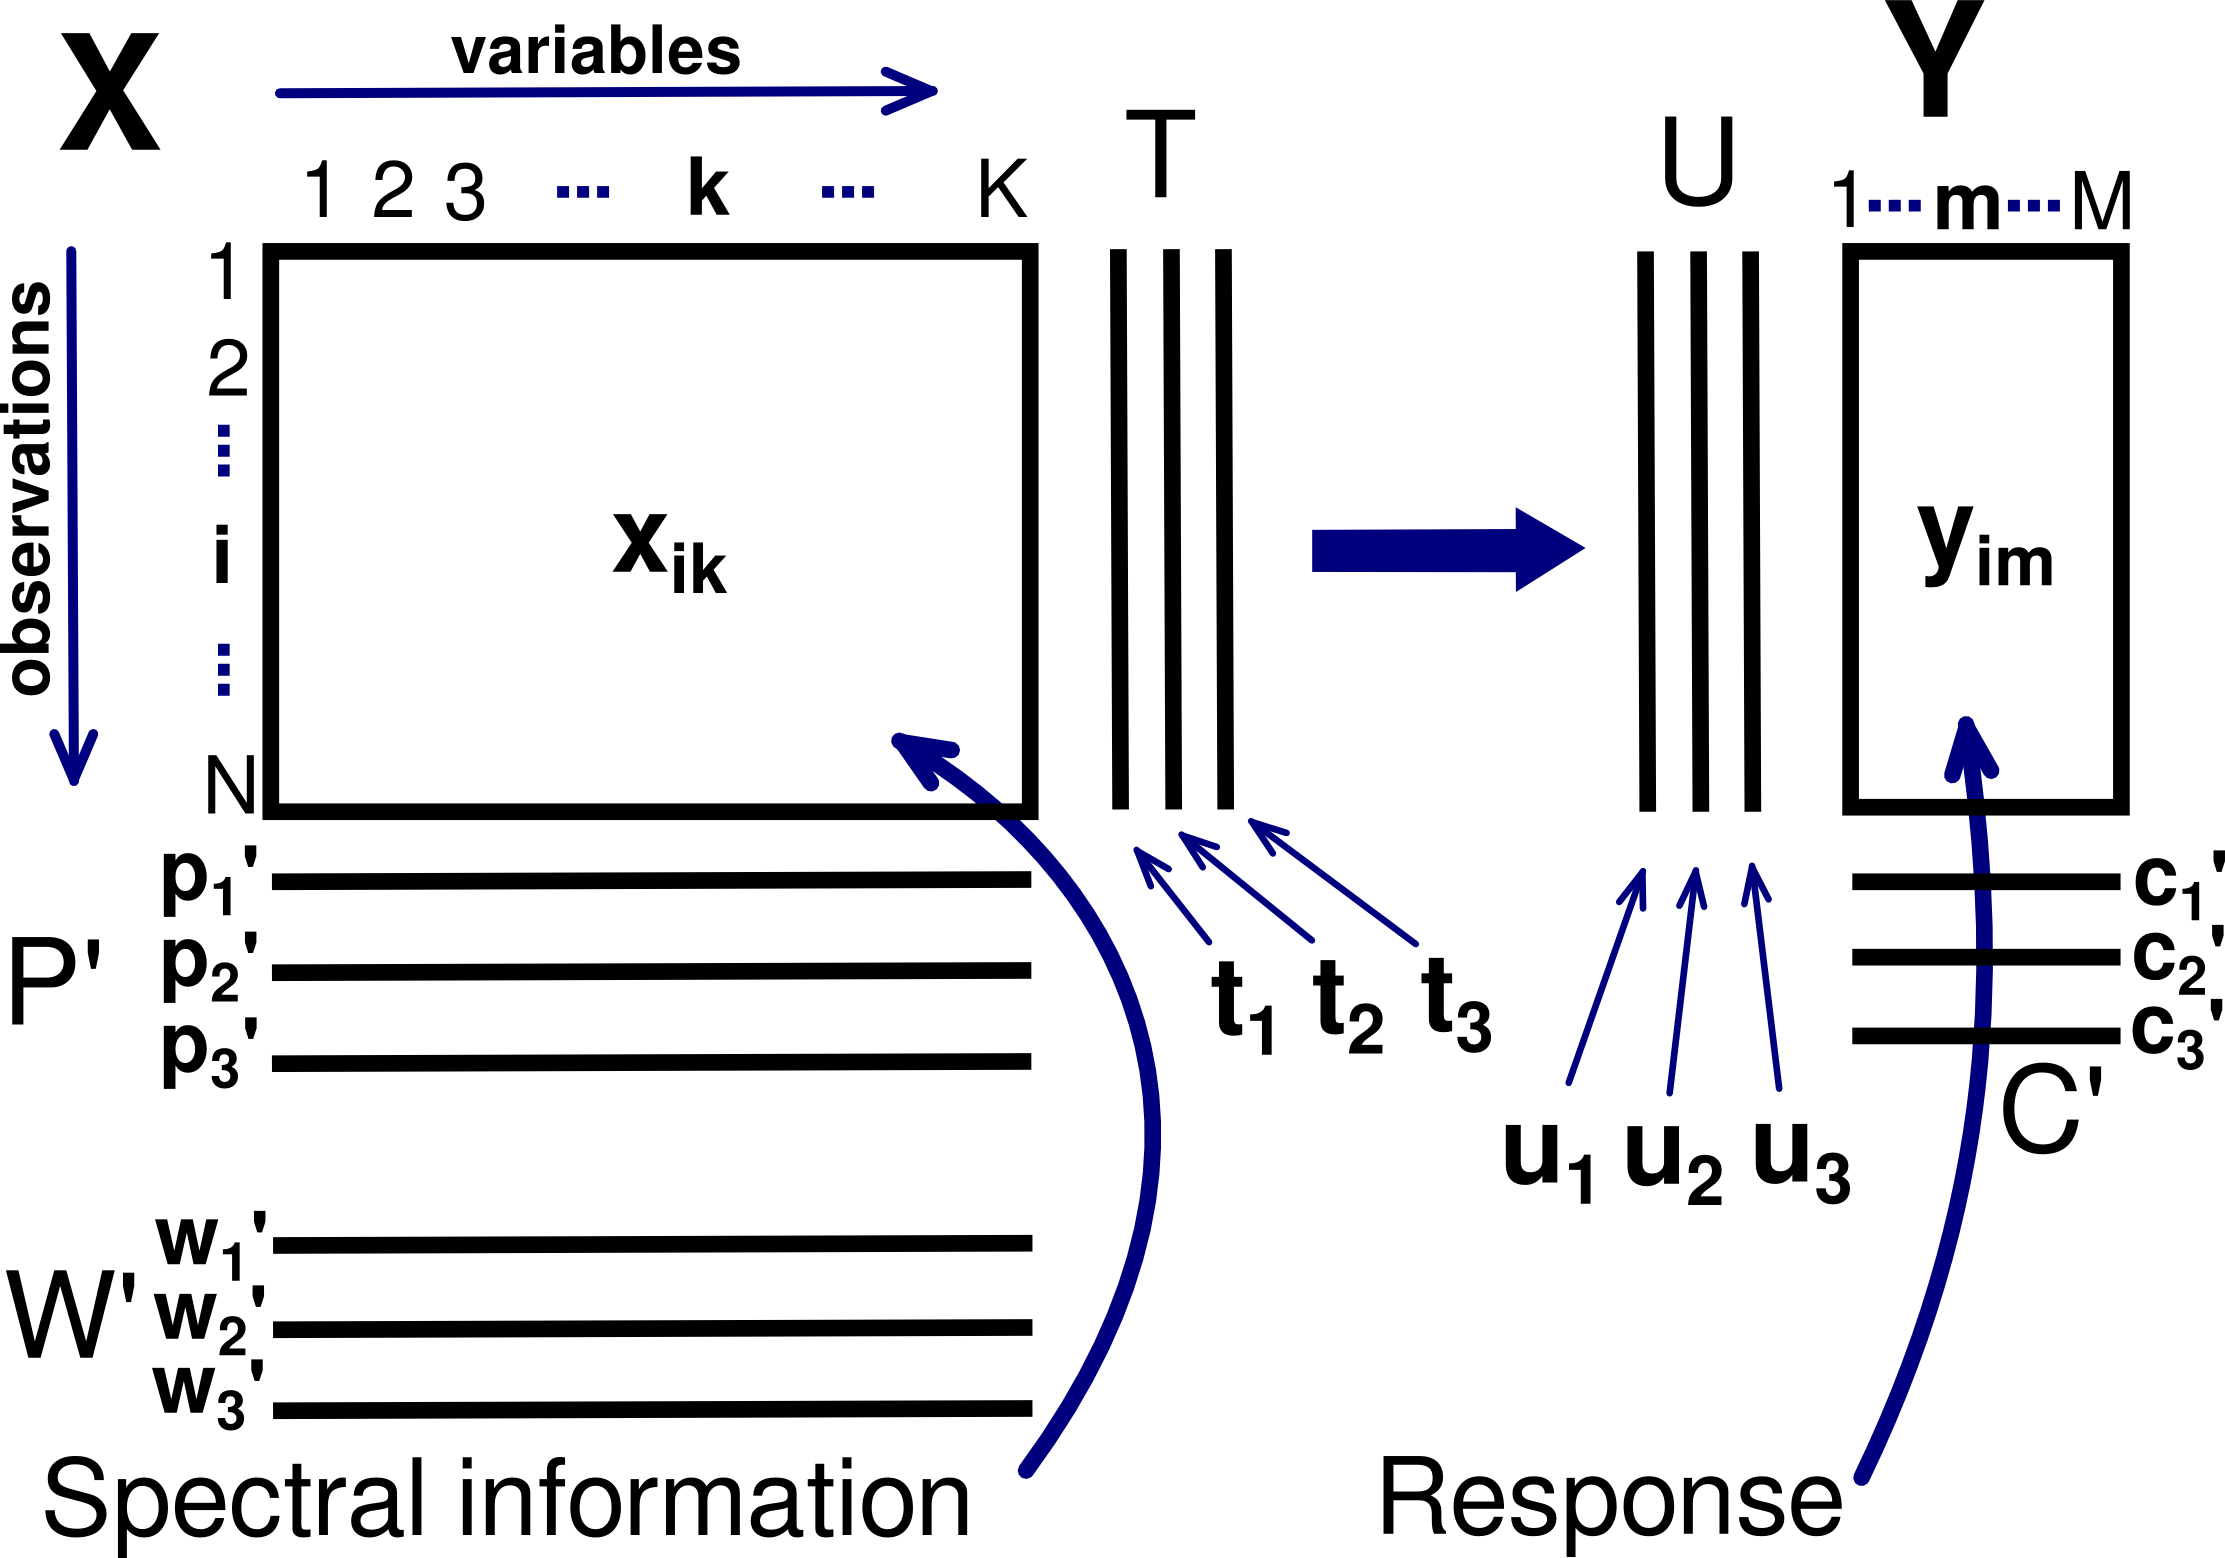
\includegraphics[width=4in]{figs/mva/01.png}
\end{center}
\caption
      [Canonical Example of a Bilinear Modeling Problem.]{
  {\bf Canonical Example of a Bilinear Modeling Problem.}
  \\
  Illustration of a data matrix $\mathbf{X}$ and a response matrix
  $\mathbf{Y}$, as they are typically used in partial least squares
  modeling problems. In metabolomics applications, the data matrix will
  contain a set of $N$ spectra, each having $K$ variables. For supervised
  modeling problems, each observation in the data matrix is paired with a
  corresponding row in the response matrix that holds either continuously
  varying outputs or binary class memberships. The data are then decomposed
  into a small number of score vectors ($\mathbf{t}$) and loading vectors
  ($\mathbf{p}$), with corresponding weight vectors ($\mathbf{w}$) used
  to transform the observations in $\mathbf{X}$ into scores-space. The
  responses in $\mathbf{Y}$ are similarly decomposed into scores
  ($\mathbf{u}$) and loadings ($\mathbf{c}$). Tick marks denote
  transposition.
}
\end{figure}

\section{Multivariate Datasets}

\begin{doublespace}
In the majority of cases, multivariate datasets used in metabolomics take the
form of second-order tensors in $\mathbb{R}^{N \times K}$. More simply, these
datasets are real matrices having $N$ rows and $K$ columns. By convention,
the data are arranged as $N$ observation row vectors of length $K$, where $K$
is referred to as the dimensionality of the dataset (Figure 3.1). Typical
examples of 1D datasets include sets of \hnmr{} or \cnmr{} NMR spectra
\cite{beckonert:nprot2007,koh:colon2009}, direct-injection mass spectra
(DI-MS, \cite{castrillo:phch2003,southam:anchem2007,zhou:asms2010}), infrared
(IR) and Raman spectra \cite{ellis:analyst2006,cherney:anchem2007}, or
capillary electrophoretograms (CE, \cite{ramautar:trac2006}). This remarkable
diversity of instrumental platforms used in metabolomics is traceable to the
ability of bilinear factorizations such as principal component analysis
(PCA, \cite{jolliffe2002}) and partial least squares (PLS, \cite{wold1993}) to
directly accept these second-order tensors for modeling (vide infra).
\\\\
The dimensionality of a multivariate dataset may be increased by adding another
``mode'', resulting in a third-order (or higher) tensor
($\mathbf{X} \in \mathbb{R}^{N \times K_1 \times K_2}$, Figure 3.2). In such
cases, the total dimensionality of the dataset is now the product of the
dimensionalities along each mode of the data tensor (e.g. $K_1 \times K_2$).
Third-order tensors are the natural data structures for sets of two-dimensional
observations, including \hhnmr{}, \hcnmr{} and \hnnmr{} NMR spectra, hyphenated
chromatography-mass spectra (LC-MS, GC-MS), hyphenated electrophoresis-mass
spectra (CE-MS), and hyphenated ion-mobility mass spectra (IM-MS). While
third-order data tensors may hold substantially more chemical information than
their second-order counterparts, they are not directly compatible with bilinear
factorization methods, and they require specialized processing,
treatment and modeling algorithms \cite{lu:ieee2009,lu:pr2011}. As an example,
tensors may be vectorized into matrices \cite{hedenstrom:cils2008} that are
suited for PCA and PLS, but at the cost of lost structural information. Methods
such as uncorrelated multilinear PCA (UMPCA, \cite{lu:ieee2009}), on the other
hand, provide a means of directly decomposing tensors into low-dimensional
spaces while maintaining structural information.
\end{doublespace}

\begin{SCfigure}
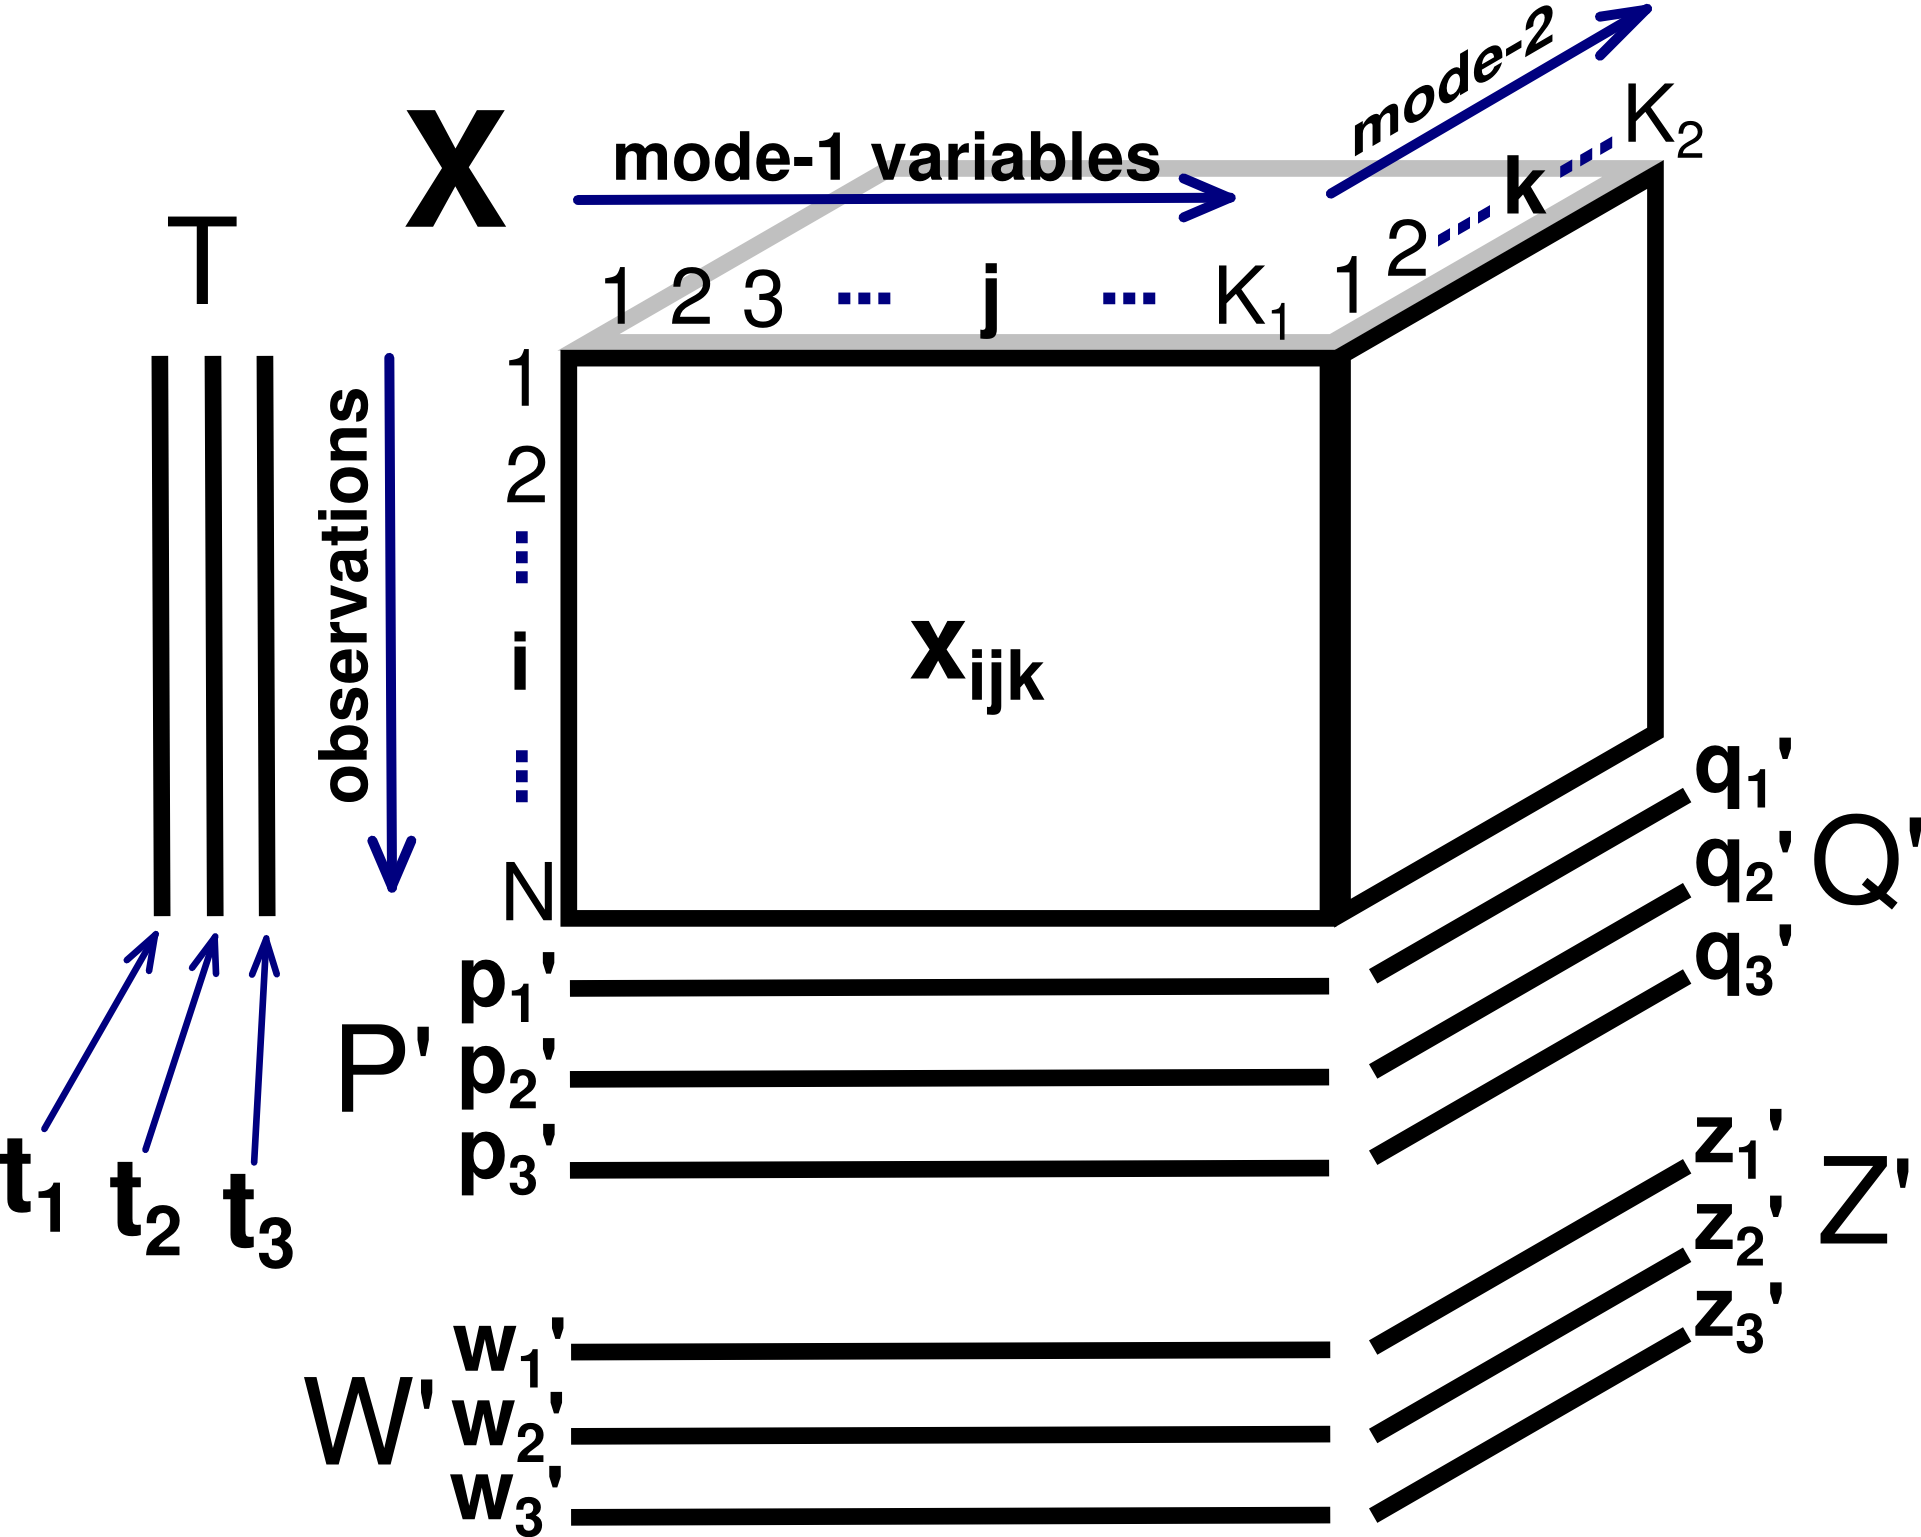
\includegraphics[width=3.5in]{figs/mva/02.png}
\caption
      [Canonical Example of an Unsupervised Trilinear Modeling Problem.]{
  {\bf Canonical Example of an Unsupervised Trilinear Modeling Problem.}
  \\
  Illustration of a third-order data tensor $\mathbf{X}$ as may be found in
  multilinear factorization problems. Such data tensors will contain a set
  of $N$ spectra, each having $K_1$ variables along their first mode and
  $K_2$ variables along their second. The data tensor is then decomposed
  into a small number of score vectors ($\mathbf{t}$) and loading vectors
  ($\mathbf{p}$, $\mathbf{q}$), with corresponding weight vectors
  ($\mathbf{w}$, $\mathbf{z}$) used to transform the observations in
  $\mathbf{X}$ into scores-space. Tick marks denote transposition.
}
\end{SCfigure}

\begin{figure}[hb!]
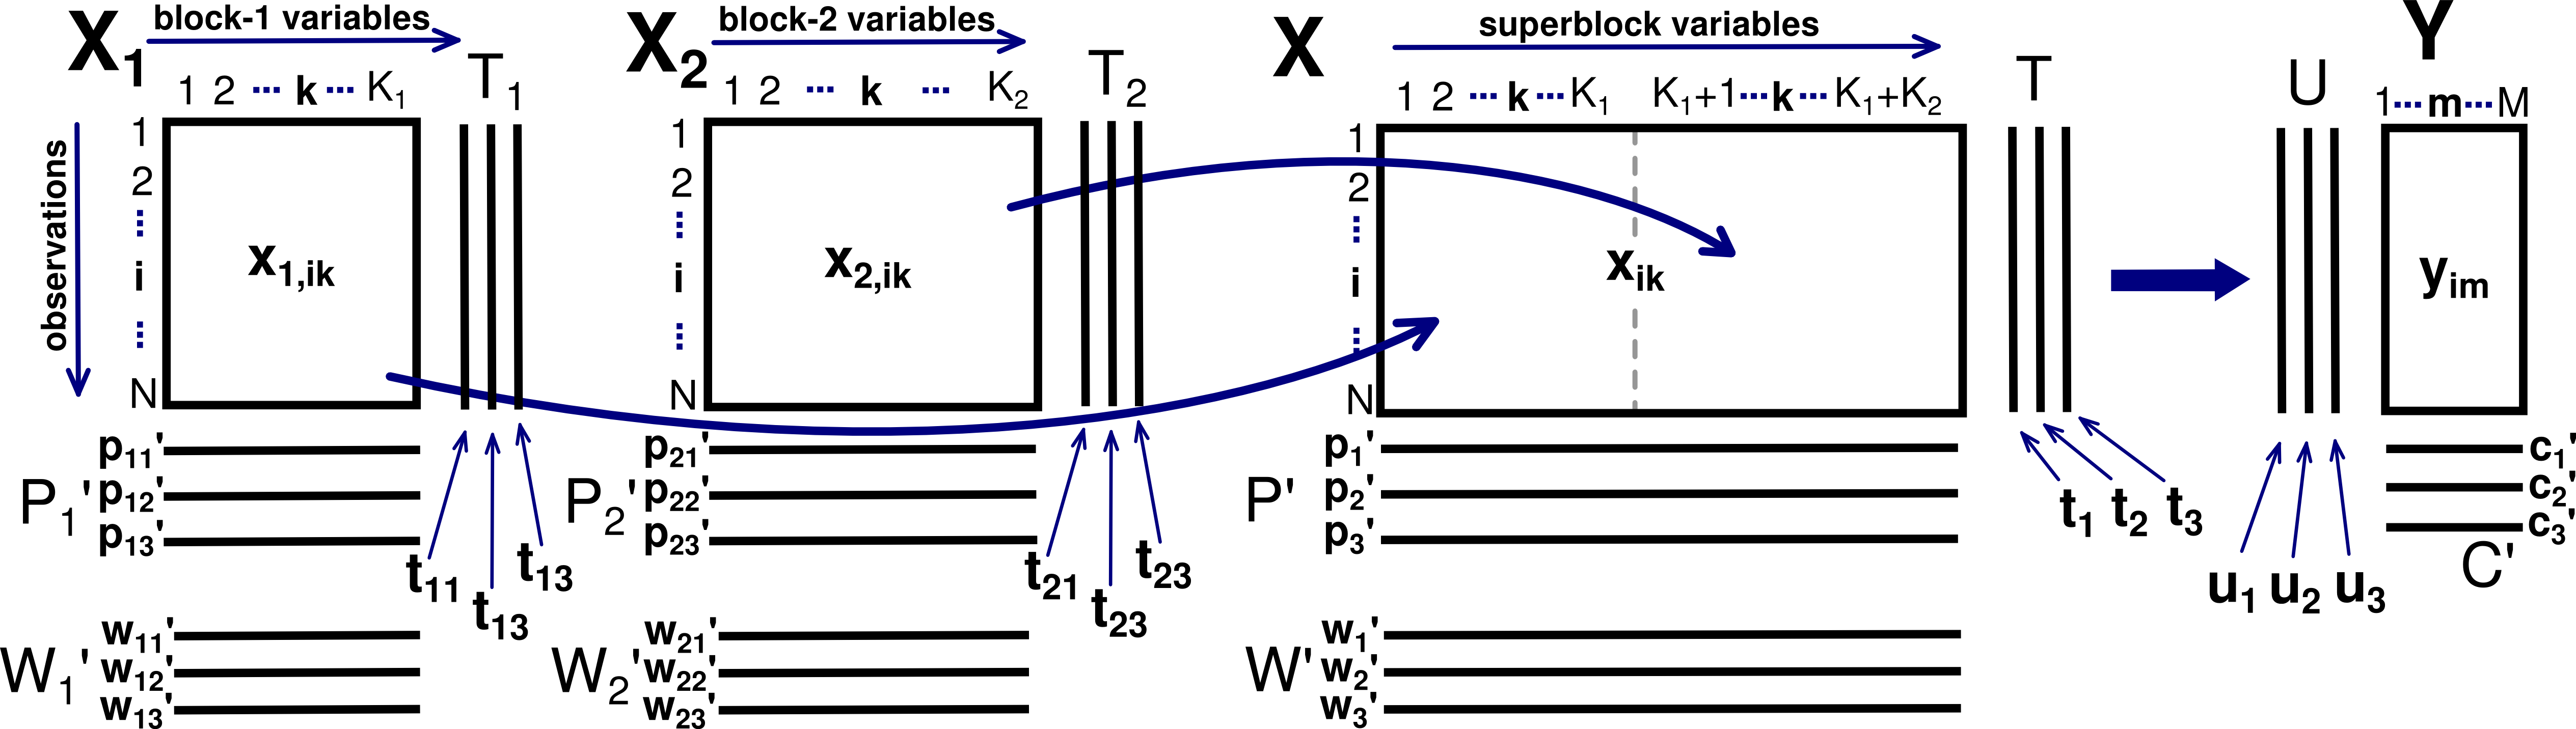
\includegraphics[width=6.5in]{figs/mva/03.png}
\caption
      [Canonical Example of a Multiblock Bilinear Modeling Problem.]{
  {\bf Canonical Example of a Multiblock Bilinear Modeling Problem.}
  \\
  Illustration of a pair of data matrices $\mathbf{X_1}$ and $\mathbf{X_2}$,
  their observation-wise concatenation $\mathbf{X}$, and a response matrix
  $\mathbf{Y}$, as they are typically used in multiblock partial least squares
  modeling problems. In metabolomics applications, each data matrix
  $\mathbf{X_b}$ in the set of $B$ matrices will contain a set of $N$ spectra,
  each having $K_b$ variables. The data are then decomposed into a small number
  of superblock score vectors ($\mathbf{t}$) and superblock loading vectors
  ($\mathbf{p}$), with corresponding superblock weight vectors ($\mathbf{w}$).
  Each individual data matrix is also decomposed into a set of block scores
  ($\mathbf{t_b}$), block loadings ($\mathbf{p_b}$) and block weights
  ($\mathbf{w_b}$). Tick marks denote transposition.
}
\end{figure}

\begin{doublespace}
Another mechanism of increasing the information content of datasets entering
into multivariate chemometric models is to collect spectral observations on
two or more complementary instrumental platforms for each sample. In such a
``multiblock'' modeling approach, each data block $\mathbf{X_b}$ contains $N$
$K_b$-variate observations \cite{westerhuis:jchemo1998,smilde:jchemo2003}.
Bilinear methods such as consensus PCA (CPCA), hierarchical PCA and PLS, and
multiblock PLS may then be used to provide information about data variation
that is correlated between data blocks. Recent examples of multiblock modeling
in metabolomics include fusions of near-IR and mid-IR spectra
\cite{bras:cils2005}, \hnmr{} NMR and direct injection electrospray mass
spectra (DI-ESI-MS, \cite{marshall:metab2015}), and observations from multiple
sensors in process control applications \cite{ferreira:jchemo2010}.
\end{doublespace}

\section{Spectral Processing}

\begin{doublespace}
Following the acquisition of experimental data, instrumentation-specific
processing must be applied to transform the data into a suitable set of
real matrices for bilinear modeling, or tensors for multilinear modeling.
Because the majority of data presented herein originated from an NMR
spectrometer, and because NMR spectra present unique challenges to the
analyst during data handling, the following discussions will center around
processing of 1D and 2D NMR datasets.
\end{doublespace}

\subsection{NMR Signals}

\begin{doublespace}
Modern NMR spectrometers effectively acquire a rotating-frame free induction
decay (FID) through the use of quadrature phase detection of the incoming
signal \cite{levitt2008}. This detection method imparts relative phase
information to the time-domain decays by creating an ``in-phase'' signal
component $i(t)$ and a ``quadrature'' component $q(t)$ phased ninety degrees
from $i(t)$. Indirect dimensions of multidimensional NMR experiments are also
collected in quadrature through interleaved acquisition of one-dimensional
decays that have been cosine- and sine-modulated by the indirect-dimension
signals \cite{states:jmr1982}. As a result, each data point in a
$D$-dimensional NMR signal collected in complete quadrature exists in a
hypercomplex space $\mathbb{H}_D$ \cite{schuyler:jmr2013}, which is defined by
a real basis element and $D$ complex basis elements:

\begin{equation}
\Phi_D \equiv \{ 1 \cdot u_1 \cdots u_D \}
\end{equation}

where multiplication by any complex element $u_d$ results in a ninety degree
phase shift in dimension $d$, and the basis elements combine commutatively
under multiplication, as follows:
\begin{align}
u_i u_j =& u_j u_i \\
u_i^2 =& -1
\end{align}

The basis elements in $\Phi_D$ are a generating set for the complete set of
components of the hypercomplex space $\mathbb{H}_D$. For example, in three
dimensions:

\begin{equation}
\Phi_3 = \{ 1, u_1, u_2, u_1 u_2, u_3, u_1 u_3, u_2 u_3, u_1 u_2 u_3 \}
\end{equation}

A scalar in $\mathbb{H}_D$ is then expressed as a linear combination of this
component set. For the three-dimensional example:

\begin{equation}
x = a + b u_1 + c u_2 + d u_1 u_2
  + e u_3 + f u_1 u_3 + g u_2 u_3 + h u_1 u_2 u_3
\end{equation}

or, more generally and succinctly:

\begin{equation}
x = \sum_{\phi \in \Phi_D} x \{ \phi \} \cdot \phi
\end{equation}

where $x\{\phi\}$ denotes the real coefficient of $x$ that scales the basis
component $\phi$ in $x$. For the above three-dimensional example, the
expression $x\{u_1 u_3\}$ would evaluate to $f$. Finally, the expression of
hypercomplex tensors is formally accomplished by defining each coefficient
as a real tensor of appropriate size, like so:

\begin{equation}
x \{ \phi \} \in \mathbb{R}^{k_1 \cdots k_K} \quad \forall \phi \in \Phi_D
\end{equation}

where $K$ is the number of modes of the tensor. The above equation may be
compactly written as $\mathbb{H}_D^{k_1 \cdots k_K}$. Any scalar
in $\mathbb{H}_D$ -- and therefore any data point in a $D$-dimensional
quadrature-complete NMR dataset -- shall require $2^D$ real coefficients
in order to be completely determined. While the hypercomplex
algebras $\mathbb{H}_0$ and $\mathbb{H}_1$ are isomorphic to the real 
($\mathbb{R}$) and complex ($\mathbb{C}$) numbers, respectively, $\mathbb{H}_2$
and $\mathbb{H}_3$ are {\it not} isomorphic to the quaternions and octonions,
as the latter are noncommutative under multiplication. This hypercomplex
algebra, introduced for partial-component nonuniform subsampling by Schuyler
et al. \cite{schuyler:jmr2013}, provides an elegant formalism for expressing
and handling NMR data.
\\\\
Mathematically, 1D NMR free induction decays are described by the following
commonly used parametric signal model:

\begin{equation}
f(t) = \sum_{m=1}^M \alpha_m \exp\left\{
  u_1 (\omega_m t + \theta_m) - \rho_m t
  \right\}
\end{equation}

where $\alpha_m$, $\omega_m$, $\theta_m$ and $\rho_m$ represent the amplitude,
frequency, phase error and decay rate of the $m$-th damped complex exponential
in the model $f(t)$. Using the above formalism for hypercomplex tensors, this
signal model is trivially extended to any number of dimensions by multiplying
in a modulation term for each dimension:

\begin{equation}
f(\mathbf{t}) = \sum_{m=1}^M \alpha_m \prod_{d=1}^D \exp\left\{
  u_d (\omega_{m,d} t_d + \theta_{m,d}) - \rho_{m,d} t_d
  \right\}
\end{equation}

For example, a 2D FID may be modeled as follows:

\begin{equation}
f(t_1, t_2) = \sum_{m=1}^M \alpha_m \exp\left\{
  u_1 (\omega_{m,1} t_1 + \theta_{m,1}) +
  u_2 (\omega_{m,1} t_2 + \theta_{m,2}) -
  \rho_{m,1} t_1 - \rho_{m,2} t_2
  \right\}
\end{equation}

In short, NMR free induction decays may be treated as sums of damped
hypercomplex exponentials. While it is possible to directly parameterize
$f(\mathbf{t})$ using either maximum likelihood estimation
\cite{chylla:jbnmr1995,chylla:jbnmr1998,chylla:anchem2011} or Bayesian
model selection and estimation
\cite{bretthorst:jmr1990a,
      bretthorst:jmr1990b,
      bretthorst:jmr1990c,
      chylla:jbnmr1993}, this chapter will focus on the soft modeling of
multiple NMR spectra using bilinear matrix factorizations. However, the above
parametric description of NMR data is useful in understanding various
processing tasks required by these hypercomplex tensors.
\end{doublespace}

\subsection{Time-domain Processing}

\begin{doublespace}
Processing of acquired NMR data is broken into two stages, where time-domain
data is manipulated, transformed into the frequency domain, and further
processed using frequency-domain functions \cite{hoch1996}.
The most routinely used time-domain NMR processing function -- and the first
to be applied during processing -- is referred to as apodization, where the
free induction decay tensor is multiplied point-wise by a window function
$w(\mathbf{t})$ that varies over $\mathbf{t}$. Multiplication by this window
function serves several purposes, including noise reduction, resolution
enhancement, shaping of individual resonances and removal of $\sin(x)/x$
truncation artifacts in the frequency domain. During apodization, it is also
common practice to selectively scale the first collected data point in an
attempt to reduce later frequency-domain baseline distortions
\cite{stoch:jmr2005,ebel:jmr2006}.
\\\\
Following apodization, one or more dimensions of the time-domain NMR data may
be extended with zeros, a process known as zero-filling. Doubling of the number
of data points by zero-filling is a well-established method of increasing both
the digital resolution and the signal-to-noise ratio (SNR) of an NMR signal,
and further zero-filling only achieves a smoother interpolation of signals in
the frequency domain \cite{ebel:jmr2006}. A final use of zero-filling is to
augment the size of a given dimension into a power of two, enabling the use of
a fast Fourier transform (FFT, \cite{cooley:mcomp1965}) in lieu of the slower
discrete Fourier transform (DFT) to move the data into the frequency domain.
\end{doublespace}

\subsection{Frequency-domain Processing}

\begin{doublespace}
When NMR free induction decays have been digitized on a grid of uniformly
spaced time-domain points, the most convenient method of transforming them
into the frequency domain is the discrete Fourier transform (DFT,
\cite{bretthorst:cmr2008,schuyler:jmr2013}). Using the introduced formalism for
hypercomplex NMR data, the DFT along dimension $d$ of a time-domain vector
$\mathbf{f} \in \mathbb{H}_D^N$ is defined as:

\begin{equation}
\mathbf{s}_k = \frac{1}{\sqrt{N}} \sum_{n=0}^{N-1}
  \exp\left\{ -2 \pi u_d \frac{n k}{N} \right\}
  \mathbf{f}_n
  \quad \forall k \in \{ 0, 1, \dots N-1 \}
\end{equation}

which is a linear transformation
$\mathcal{F}_d : \mathbb{H}_D^N \to \mathbb{H}_D^N$. Discrete Fourier
transformation of multidimensional NMR data along one dimension requires the
application of $\mathcal{F}_d$ to every $d$-mode vector of the hypercomplex
tensor, and full Fourier transformation requires such an operation along each
mode of the tensor. Discrete Fourier transformation is computationally
efficient when using the FFT, and requires no prior knowledge about the
frequency content of the data. However, when only a subset of data points
have been collected from a uniform Nyquist grid, as is the case during
nonuniform sampling (NUS), the DFT is a sub-optimal estimator of frequency
content, and other non-Fourier methods of transformation are required
\cite{bretthorst:cmr2008,mobli:pnmrs2014}.
\\\\
Once transformed into the frequency domain, NMR spectra require a phase
correction processing step, in which a phase factor $\Theta(\omega)$ is
multiplied point-wise with the data to correct for phase errors
(i.e. $\theta_{m,d}$ terms in $f(\mathbf{t})$) in the data. For example, a
1D phase-factor along dimension $d$ would have the following form:

\begin{equation}
\Theta(\omega) = e^{ -u_d \theta(\omega) }
\end{equation}

Ideally, the detected time-domain free induction decays would arrive in-phase
with respect to the receiver, and fine tuning of acquisition parameters can
often accomplish this \cite{chylla:jbnmr1998}.
However, variations in receiver phase, dead time
between the transmit and receive gating circuits, and delays arising from
analog and digital filtering can all introduce phase errors. These phase
errors mix the in-phase and quadrature components of the hypercomplex signal,
and produce a mixture of desirable absorptive spectral lines and broad
dispersive lines between the real and imaginary components of each data point.
Unmixing of these absorptive and dispersive contributions to the real spectral
component involves the identification of the phase error $\theta(\omega)$, an
expansion of phase error terms as powers of $\omega$:

\begin{equation}
\theta(\omega) = \theta_0 + \theta_1 \omega + \theta_2 \omega^2 + \dots
\end{equation}

Realistically, phase errors higher than first-order are not observed in modern
NMR spectra, and phase correction rests on the determination of a zero-order
phase error ($\theta_0$) and a first-order phase error ($\theta_1$) in each
dimension. This determination may be performed manually, through
software-interactive adjustment of zero- and first-order corrections by the
analyst. However, manual phase correction is generally too time-consuming in
the case of chemometric studies, where there are tens to hundreds of spectra
to correct. In that case, the task of phase correction is handed to any number
of automated routines that correct each spectrum individually. Spectra may be
automatically phase-corrected by maximization of the most negative absorptive
data point \cite{siegel:aca1981}, analysis of the absorption-versus-dispersion
\cite{craig:jmr1988} or symmetry \cite{heuer:jmr1991} characteristics of
spectral lines, baseline optimization \cite{brown:jmr1989} or entropy
minimization \cite{chen:jmr2002}, to name a few. It is important to note that,
when the ultimate fate of the spectral data is multivariate analysis, the
phase-correction of each spectrum in isolation is wasteful of information that
is available from treating the dataset as an ensemble \cite{worley:cils2014},
as phase differences {\it between} spectra non-linearly affect both line shapes
and baseline, possibly emphasizing spectral details that contain no
chemically or biochemically relevant information.
\end{doublespace}

\section{Statistical Treatment}

\begin{doublespace}
The properties of the bilinear factorizations commonly applied in metabolomics
dictate that processed data tensors be treated by one or more operations before
they are suitable for modeling. These statistical treatments generally aim to
either reduce the dimensionality of the data tensor (i.e. binning and variable
selection) or increase the self-consistency of observations and variables
(i.e. alignment, normalization and scaling). Treatment operations are usually
instrumentation-agnostic, as the data at this stage of handling almost always
fall into one of the general structures outlined in
\hyperlink{section.3.2}{Section 3.2}.
\end{doublespace}

\subsection{Binning}

\begin{doublespace}
Because the chemical shifts of \hnmr{} nuclei depend strongly on temperature,
pH, ionic strength, and several other factors that affect their electronic
environment, spectral datasets acquired for NMR metabolic fingerprinting
suffer from imprecision in \hnmr{} chemical shifts between observations.
This chemical shift imprecision, known as a problem of imperfect correspondence
among variables in $\mathbf{X}$ \cite{aberg:abc2009}, decreases the reliability
and interpretability of multivariate bilinear models (e.g. PCA, PLS) trained
directly on full-resolution spectral data in $\mathbf{X}$. Similar errors in
correspondence may also occur in chromatographic datasets, where small drifts
in retention time arise from instrumental instability, analyte interactions,
and fluctuations in mobile phase and stationary phase composition
\cite{nielsen:jchrom1998}. The traditional method of mitigating imperfect
variable correspondence in a data matrix is to partition the original set
of variables into a smaller set of regions, referred to as bins, and
to integrate each bin to yield a data matrix having reduced dimensionality.
\\\\
While binning masks variable mis-correspondence, filters incoherent
instrumental noise, and achieves substantial dimensionality reduction, it often
hides potentially significant variation in low-intensity resonances nearby
strong signals. If bin regions are specified with a uniform size, binning is
nearly guaranteed to split signals or spectral features into multiple bins,
resulting in undesirable multicollinearities within the reduced variable set.
Optimized binning \cite{sousa:cils2013} attempts to avoid dividing signals
between bins by adjusting uniform bin boundaries into local minima of the
data matrix mean, $\langle\mathbf{X}\rangle$. However, because optimized
binning begins with a uniform bin set, its practical ability to minimize peak
splitting is limited. More complex methods of region identification use either
peak detection \cite{davis:cils2007} or recursive subdivision
\cite{demeyer:anchem2008} in order to define a more optimal bin set without
relying on uniform bin boundaries.
\end{doublespace}

\subsection{Alignment}

\begin{doublespace}
Binning capably masks variability in signal positions and provides an effective
means of dimensionality reduction, but it also results in a drastic loss of
fine spectral information, as nearby distinct spectral features have been
integrated together in the binning process. When full spectral resolution is
required during model training and interpretation, the correspondence problem
in NMR and chromatographic datasets may be alternatively addressed by signal
alignment methods. The most commonly applied alignment algorithms rely on
either a warping transformation
\cite{nielsen:jchrom1998,
      forshed:aca2003,
      wu:jcim2006} or linear shifts
\cite{veselkov:anchem2009,
      savorani:jmr2010,
      tomasi:jchrom2011} to bring individual variables of each observation
into alignment with a reference observation, which is usually the mean of
the data. Warping during alignment is more applicable in situations where
a linear dependence between variable index (e.g. retention time) and peak
width is expected. In contrast, shift-based alignment preserves peak width,
which is ideal for spectroscopic datasets. Like binning, all alignment
algorithms must first subdivide the variable set into regions that are then
individually warped or shifted, and considerations similar to those in
binning apply equally well during alignment region selection.
\end{doublespace}

\subsection{Normalization}

\begin{doublespace}
Despite the quantitative nature of most spectroscopic platforms, chemometric
samples exhibit variable total analyte concentrations due to variations in
sample preparation, instrument stability, or even the samples themselves.
These ``dilution errors'' are especially common in metabolomics experiments
using samples of biofluids such as urine, where total concentrations may vary
several orders of magnitude. To ensure spectral intensities in a data tensor
are directly comparable across each observation, normalization is applied to
the tensor \cite{worley:cmb2013}. The most common normalization method used in
chemometrics is unit-integral or constant-sum (CS) normalization, where each
observation is scaled such that its total integral is unity
\cite{craig:anchem2006}. CS normalization does more harm that good, however,
as it introduces false correlations between variables and poorly tolerates
large disparities in intensities between each observation.
\\\\
In an attempt to overcome the drawbacks of CS normalization, Dieterle et al.
introduced probabilistic quotient (PQ) normalization, in which the median
normalization quotient between all corresponding data points is used as an
estimator of the true dilution factor \cite{dieterle:anchem2006}. Shortly
after, a method of normalization based on intensity histogram matching (HM)
was proposed as an alternative to PQ normalization, taking cues from image
processing algorithms \cite{torgrip:metab2008}. Based on their ability to
more accurately recover true dilution factors, both PQ and HM normalization
were reported to outperform CS normalization on real and simulated \hnmr{}
NMR metabolomics data matrices. Finally, while more commonly applied to
IR spectroscopic data, standard normal variate (SNV) and its mathematical
cousin, multiplicative scatter correction (MSC) are also candidate methods
for normalizing data tensors produced by NMR and other spectroscopic
platforms \cite{fearn:cils2009}.
\end{doublespace}

\subsection{Scaling}

\begin{doublespace}
Because bilinear factorization methods such as PCA and PLS generate models
based on the eigenstructure of the covariance matrices of $\mathbf{X}$ and
$\mathbf{Y}$ (vide infra), they are sensitive to the magnitudes of individual
variables in those matrices. Variables with greater intensity -- and therefore
greater variance -- in a data matrix will draw the attention of these methods,
resulting in an unequal weighting of variable importance during model training
\cite{jolliffe2002,smilde:anchem2005,vandenberg:bmcg2006}. As a consequence,
analysts commonly apply one or more scaling transformations to their data prior
to modeling. The simplest and most pervasive method, referred to as Unit
Variance (UV) scaling, centers each variable with respect to its mean and
scales by its standard deviation, like so:

\begin{equation}
\tilde{x}_{nk} = \frac{x_{nk} - \bar{x}_k}{s_k}
\end{equation}

where $\widetilde{\mathbf{X}}$ is the scaled data matrix, $\bar{x}_k$ is the
sample mean of the $k$-th variable over all $N$ observations, and $s_k$ is the
corresponding sample standard deviation. Subtraction of the sample mean
facilitates the identification of differences between observations, and
scaling by the sample standard deviation equally weights every variable
in $\mathbf{X}$. When data are UV-scaled, methods that normally analyze
covariance eigenstructure will instead rely on {\it scale-invariant}
correlations between variables. Although UV scaling achieves an equal weighting
of all variables entering into PCA or PLS, it amplifies the weight of noise
variables relative to that of signal variables, resulting in decreased model
utility and reliability \cite{hoefsloot:jchemo2006}. Pareto scaling applies a
less aggressive scaling than UV by retaining partial covariance between
variables in an attempt to reduce this noise amplification:

\begin{equation}
\tilde{x}_{nk} = \frac{x_{nk} - \bar{x}_k}{\sqrt{s_k}}
\end{equation}

A more advanced scaling method that avoids noise amplification uses a maximum
likelihood scaling transformation (MALS, \cite{hoefsloot:jchemo2006}) that
accounts for the estimated distribution of noise in $\mathbf{X}$. Other forms
of scaling have been developed that emphasize various desirable features in
a data structure. For example, {\it va}riable {\it st}ability (VAST) scaling
multiplies each element by the coefficient of variation of its variable in
order to focus on highly stable spectral features:

\begin{equation}
\tilde{x}_{nk}
 = \frac{x_{nk} - \bar{x}_k}{s_k} \cdot
   \frac{\bar{x}_k}{s_k}
\end{equation}

The alternative level scaling method scales data elements by their sample mean,
effectively focusing later analyses on changes in relative magnitude:

\begin{equation}
\tilde{x}_{nk} = \frac{x_{nk} - \bar{x}_k}{\bar{x}_k}
\end{equation}

However, both VAST and level scaling have a more limited scope of
application than the general UV, Pareto and MALS methods described above, as
they yield optimal transformations only on data structures containing the
features they aim to accentuate. For example, VAST scaling is not suited for
data tensors that contain large variation between experimental groups, unless
further steps are taken to VAST-scale on a (supervised) per-group basis.
\\\\
A special case for scaling occurs during multiblock modeling when two or more
data blocks contain differing variable counts. In these situations, data blocks
having more variables would acquire a larger effective weight during model
training. For example, joint modeling of full-resolution \hnmr{} NMR data
($K \approx 10^3$) and mass spectral data ($K \approx 10^5$) would result in
a weighting of MS variables by a factor of ten relative to NMR variables. To
achieve equal block weighting, the variables of each block must be scaled by
the square root of the number of block variables:

\begin{equation}
\tilde{\tilde{x}}_{bnk} = \frac{\tilde{x}_{bnk}}{\sqrt{K_b}}
\end{equation}

where the second tilde indicates block scaling in addition to any standard
scaling (e.g. UV, Pareto) that may have been applied. When all data blocks
contain analyte concentrations instead of raw spectral variables, range
scaling may be applied prior to block scaling to remove instrumental response
factors and transform all concentrations into relative values
\cite{smilde:anchem2005}:

\begin{equation}
\tilde{x}_{bnk}
 = \frac{x_{bnk} - \bar{x}_{bk}}
        {\max_n(x_{bnk}) - \min_n(x_{bnk})}
\end{equation}

Range scaling holds intuitive appeal for multiblock modeling of concentration
data, but its application to other kinds of datasets is ill-advised, as it
suffers from similar noise amplification problems as UV scaling.
\end{doublespace}

\subsection{Variable Selection}

\begin{doublespace}
Due to the expense of sample preparation and data acquisition in metabolomics
studies, a strong temptation exists to retain all observed variables during
multivariate analyses \cite{kjeldahl:jchemo2010}. Because variables are scaled
to equal (or nearly equal) weight prior to modeling, this practice produces
multivariate models that suffer in both predictive ability and general
reliability. In short, only variables that are truly relevant to the chemical
system under study should be included during modeling. To that end,
conservative manual removal of irrelevant variables based on spectroscopic
and biochemical domain knowledge is often performed in metabolomics. \hnmr{}
NMR datasets, for instance, nearly always contain highly varying signals from
solvents, buffers, and chemical shift reference compounds, all of which may
confound or overshadow relevant sources of variation. Variables containing
such signals, as well as signal-free variables that only contain instrumental
noise, are excellent candidates for manual variable selection. More
computationally intensive methods of variable selection, including support
vector machine recursive feature elimination (SVM-RFE), genetic algorithms
(GA), random forests (RF) and bootstrapping have also been developed to more
aggressively select variables from multivariate data structures
\cite{lin:metab2011,wongravee:anchem2009}. While it is important to retain
only relevant variables for modeling, an over-aggressive variable selection
is equally detrimental, as it leads to over-fit models that may fail to
tolerate subsequent outlying observations.
\end{doublespace}

\section{Modeling}

\begin{doublespace}
The most widely applied modeling methods in metabolomics -- namely principal
component analysis, partial least squares and orthogonal projections to latent
structures (OPLS, \cite{trygg:jchemo2002}) -- fall within a class of methods
known as bilinear matrix factorizations. The general form of a bilinear matrix
factorization is:

\begin{equation}
\mathbf{X} = \mathbf{T} \mathbf{P}^T + \mathbf{E}
\end{equation}

where the data matrix $\mathbf{X} \in \mathbb{R}^{N \times K}$ is approximated
by the product of two matrices, $\mathbf{T} \in \mathbb{R}^{N \times A}$ and
$\mathbf{P} \in \mathbb{R}^{K \times A}$, which are referred to as ``scores''
and ``loadings'', respectively. The matrix
$\mathbf{E} \in \mathbb{R}^{N \times K}$ holds any variation in $\mathbf{X}$
that is not captured by the scores and loadings. To understand how such a
factorization may be used to approximate a data matrix, it is instructive to
consider the product of scores and loadings in vector form:

\begin{equation}
\mathbf{X} = \sum_{a=1}^A \mathbf{t_a} \mathbf{p_a}^T + \mathbf{E}
\end{equation}

where $\mathbf{t_a}$ and $\mathbf{p_a}$ are the $a$-th columns of the score
and loading matrices, respectively. In other words, the data matrix is
approximated by a set of $A$ rank-1 matrices that are constructed by the
outer products of each pair of scores and loadings. Because $A$ is commonly
much less than either $N$ or $K$, these bilinear factorizations are also
referred to as low-rank approximations of their data matrices.
\\\\
It is important to note that nearly every data matrix modeled by equation (3.x)
in metabolomics contains far fewer observations than variables
(i.e. $N \ll K$) \cite{worley:cmb2013}. In this situation, there are infinitely
many solutions to the equation that yield the same error $\mathbf{E}$. This is
easily demonstrated by multiplying the scores and loadings by an orthonormal
matrix $\mathbf{R} \in \mathbb{R}^{A \times A}$:

\begin{align}
\mathbf{X}
 =& \: \hat{\mathbf{T}} \hat{\mathbf{P}}^T + \mathbf{E}
\nonumber \\
 =& \: \mathbf{T} \mathbf{R} \mathbf{R}^T \mathbf{P}^T + \mathbf{E}
\nonumber \\
 =& \: \mathbf{T} \mathbf{P}^T + \mathbf{E}
\end{align}

where $\hat{\mathbf{T}} = \mathbf{T} \mathbf{R}$ and
$\hat{\mathbf{P}} = \mathbf{P} \mathbf{R}$. A similar expansion of the solution
set may be accomplished by multiplying the scores by a diagonal $A \times A$
matrix, and multiplying the loadings by the inverse of the same diagonal
matrix. This equivalence of an infinite number of solutions to equation (3.x),
known as the problems of rotational and scale ambiguity, is solved by placing
constraints on the values that scores and loadings may take
\cite{dejuan:aca1997,jolliffe2002}. The choice of constraints defines a
particular bilinear factorization method as unique, and determines what
kind of information is sought from a data matrix using that method.
\end{doublespace}

\subsection{Principal Component Analysis}

\begin{doublespace}
FIXME.
\end{doublespace}

\subsection{Principal Component Regression}

\begin{doublespace}
FIXME.
\end{doublespace}

\subsection{Partial Least Squares}

\begin{doublespace}
FIXME.
\end{doublespace}

\subsection{Orthogonal Projections to Latent Structures}

\begin{doublespace}
FIXME.
\end{doublespace}

\subsection{Multiblock PCA and PLS}

\begin{doublespace}
FIXME.
\end{doublespace}

\section{\hnmr{} NMR Fingerprinting of Brewed Coffees}

\begin{doublespace}
FIXME.
\end{doublespace}

\subsection{Materials and Methods}

\begin{doublespace}
FIXME.
\end{doublespace}

\subsection{Results and Discussion}

\begin{doublespace}
FIXME.
\end{doublespace}

\section{Profiling of Joint \hnmr{} NMR and DI-ESI-MS Data}

\begin{doublespace}
FIXME.
\end{doublespace}

\subsection{Materials and Methods}

\begin{doublespace}
FIXME.
\end{doublespace}

\subsection{Results and Discussion}

\begin{doublespace}
FIXME.
\end{doublespace}

\section{Monte Carlo Analysis of Scores-space Separations}

\begin{doublespace}
FIXME.
\end{doublespace}

\subsection{Materials and Methods}

\begin{doublespace}
FIXME.
\end{doublespace}

\subsection{Results and Discussion}

\begin{doublespace}
FIXME.
\end{doublespace}

\section{Conclusions}

\begin{doublespace}
FIXME.
\end{doublespace}

\bibliographystyle{abbrv}
\bibliography{bworley}

